\documentclass{article}
\usepackage{graphicx} % Required for inserting images
\usepackage{hyperref}
\usepackage{tcolorbox}
\usepackage{menukeys}


\title{The Guide To Making talkomatic.co Themes}
\author{BatteRaquette58 }
\date{August 2024}

\begin{document}

\maketitle
\tableofcontents
\clearpage

\maketitle

\section{Prerequisites}

First, you’ll need to be on a computer, and get a text editor. Technically, any editor can work, but generally, Visual Studio Code (\url{https://code.visualstudio.com/})\footnote{Consider using VS Codium if you value your privacy, as the VS Code builds on the website mentioned have telemetry.} is preferred, and is the one used in this guide.

Now that you have VS Code installed (acronym of Visual Studio Code), you will now need the \href{https://discord.com/channels/1252540401072607355/1253474521537577030/1276435400377765970}{Talkomatic index stylesheet}, which is the template for themes.

Themes are configured using a programming language called CSS (Cascading Style Sheets), however all the main concepts that you need to learn about CSS to create themes are completely explained here. Still, if you get blocked or do not understand a concept; feel free to ask a question in the forum thread, and I'll try to get back as soon as possible. ;-)
\clearpage

\subsection{How do you even apply themes?}

On the \href{https://talkomatic.co}{Talkomatic main page}, there is a button with a settings icon above the room list menu. (see Figure 1)
\begin{figure}
    \begin{minipage}{0.3\textwidth}
        \centering
        
\includegraphics[width=1\linewidth]{1.png}
        \caption{Settings button}
        \label{fig:enter-label}
    \end{minipage}\hfill
    \begin{minipage}{0.3\textwidth}
        \centering
        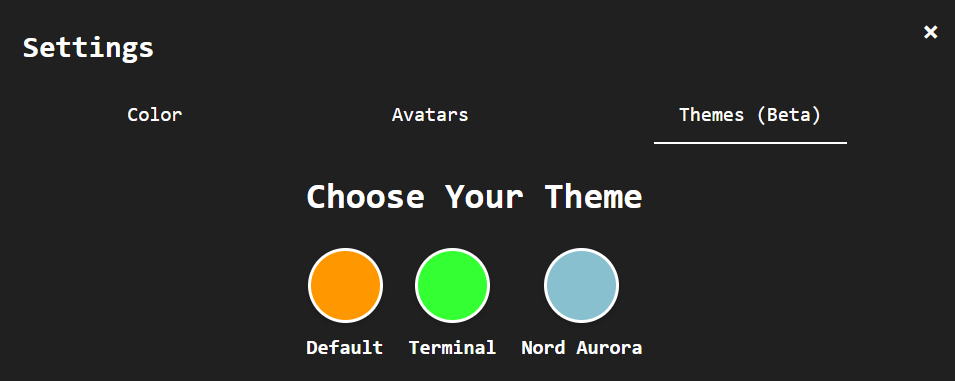
\includegraphics[width=1\linewidth]{2.png}
        \caption{Themes menu}
        \label{fig:enter-label}
    \end{minipage}\hfill
    \begin{minipage}{0.3\textwidth}
        \centering
        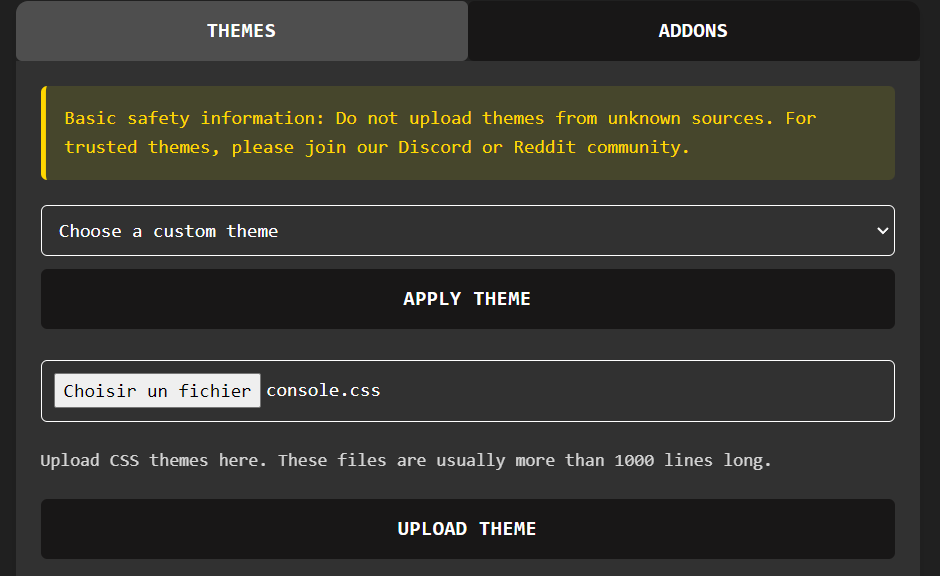
\includegraphics[width=1\linewidth]{3.png}
        \caption{Custom Themes tab}
        \label{fig:enter-label}
    \end{minipage}
\end{figure}

Click on the "Themes" tab (see Figure 2), where there should be a selection of ready-to-go themes available.

At the bottom of this tab, there should be a "Custom Themes/Addons (Advanced)" section, where if you press on the "THEMES" tab in the section, there should be a prompt like the image on Figure 3. On this tab, you can click on the "Choose file" button, where Talkomatic will ask for a .css file (stylesheet theme file) to choose. When you are done, you can simply click on "Upload theme", where the theme will be applied.
\clearpage

\section{Let's get started!}

First, open VS Code (or your editor, but this guide uses VS Code), and press \keys{\ctrl + o}\footnote{On mac, press \keys{\cmd + o}.} to open a file. This will trigger the choose file prompt, where you'll choose the template theme file you downloaded (see 1. Prerequisites). Now that you opened the template file, the editor should look like something along the lines of this (see Figure 4).
\begin{figure}
    \centering
    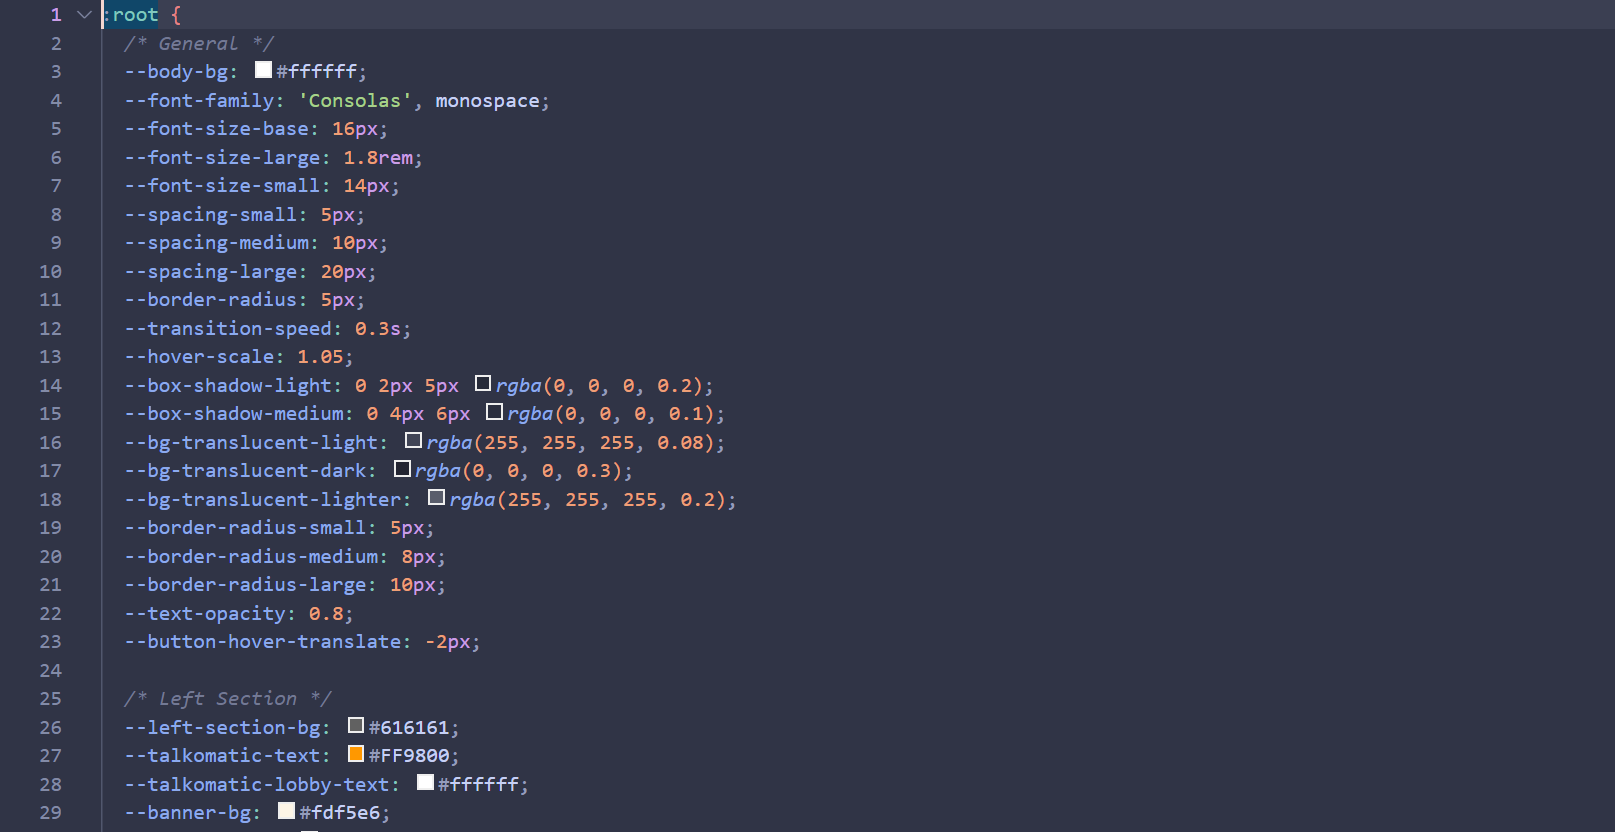
\includegraphics[width=1\linewidth]{4.png}
    \caption{organized-css.css}
    \label{fig:enter-label}
\end{figure}

For now, only focus on the \texttt{:root} section, that all have the lines that begin with \texttt{--}. These are called variables. They're a bit like in math, they have a name, and contain a value. Here, the variables can also mean a number, but also a \textcolor{blue}{colour}, and even a \textsc{font}!

\subsection{How do CSS "variables" really work? (mainly colour)}

Alright, before, we just need to know the most important thing, what are these variables, what can they contain, and how do we modify these?
By far the most type of variables used here are \textcolor{magenta}{colour variables}; here's a quick example.
\begin{tcolorbox}[colback=green!5!white,colframe=green!75!black,title=Hexadecimal colour]
  \texttt{--my-colour: \#ff0000;}
\end{tcolorbox}
\clearpage

Here, the value of this variable called "\texttt{my-colour}"\footnote{Here, the \texttt{--} just tells CSS that this is a variable.} is \textcolor{red}{\#ff0000}. This is a common way with 6 characters (7 with the \#) to represent colour that CSS understands, which you can generate using a colour picker\footnote{Either use one on the web, I recommend \url{https://coolors.co/generate} for a quick colour palette, or use the one built in VS Code (see Figure 5).} without having to know how it really works.

\begin{figure}
    \centering
    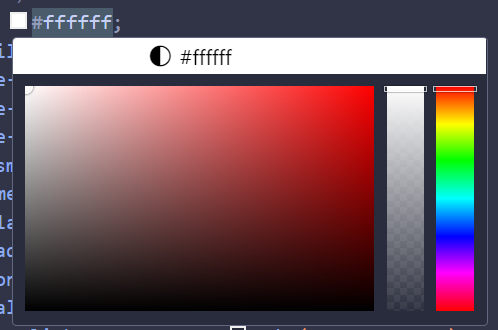
\includegraphics[width=1\linewidth]{5.png}
    \caption{VS Code colour picker (hover your mouse over a colour square)}
    \label{fig:enter-label}
\end{figure}

\begin{tcolorbox}[colback=green!5!white,colframe=green!75!black,title=\textcolor{red}{R}\textcolor{green}{G}\textcolor{blue}{B} (\textcolor{red}{Red} \textcolor{green}{Green} \textcolor{blue}{Blue}) colour]
  \texttt{--my-colour: rgb(255, 0, 0);}
\end{tcolorbox}

This the other major colour system used (this piece of code is equivalent to the previous hex example), that CSS understands. Think of the \texttt{rgb} system in CSS as a function, where you give it 3 variables, red, green, and blue variables, all ranging from 0 to 255 (255 included), where increasing the red value puts more red into the colour, decreasing the blue value puts less blue into the colour, etc. Here, \texttt{\textcolor{red}{rgb(255,\ 0,\ 0)}} is a red colour, since we've put all red colour possible in the mix, and no green nor blue colour at all. Again, a lot of colour pickers also support RGB colour, but you can always convert hexadecimal colour codes to RGB ones, and vice-versa via colour system converters. (e.g, search up "\texttt{hex to rgb}")
\clearpage

Armed with this knowledge, this is enough to do colour themes\footnote{In the "Advanced Topics" section, there is an explanation on how you can use transparent colour.}, although, we only have covered one of the main three topics, and the other two topics are explained in the "Advanced Topics" section. I think this is enough theory for now, since I don't want to bore you too much with details, so it's time to get to business, and making actual themes with this. 

\section{Modifying the template theme to make your own colour themes!}

For colour themes, we only focus on the \texttt{:root} section\footnote{The section with all the variables to configure.}, and specifically those who contain colour values\footnote{On VS Code, all colour values are marked with a square previewing its colour, with this you can identify where are all the colour variables you can tweak.}. With the little crash course from section 2.1 on colours, you can practically change any colour to your liking! Now, just a little tip so you can more easily know what variable does what:\footnote{Do not modify the variable names! Only modify their values.}

- All variables that contain "\texttt{bg}" in their name, signify that their colour is used for a background colour's value (\textbf{bg} = \textbf{b}ack\textbf{g}round).

- All variables that contain "\texttt{border}" in their name, signify that well, the value is used for a border's colour.

- All variables that contain "\texttt{hover}" in their name, signify that this is the colour used when the user is hovering over that element with their cursor.

- All variables that contain "\texttt{checked}" in their name, signify that this is the colour used when this element has been checked/chosen (e.g, a checkbox being chosen, a choice between options that Talkomatic calls "radios").

- All variables that contain "\texttt{active}" in their name, signify that this is the colour used when this element (e.g a button) has been pressed/activated.

- All variables that contain "\texttt{color}" or none of the above in their name, \textbf{usually}\footnote{Exceptions might exist.} signify that this is for the text's colour.

Now that you're all done tinkering with your new creation, be sure to press \keys{\ctrl + s}\footnote{On Mac, press \keys{\cmd + s}} in order to save your theme. To now use it, simply follow the tutorial in section 1.1 "How do you even apply themes?".
\clearpage

\section{Finding and distributing themes}

Let's say you just learned about this themes feature, and you want to use/share some, how do you even do that?
Well, you are in luck, to answer your question (\textit{shhhhhhhh}, just pretend you did ask that), there are 2 main \textbf{reputable and trustworthy}\footnote{Themes from other sources might not work, or even be malicious! The sources that I am going to name are moderated, so you can ensure that the themes are bug-free.} sources; the \href{https://reddit.com/r/talkomatic}{r/talkomatic Reddit subreddit}, or the \href{https://discord.com/channels/1252540401072607355/1275948725553860639}{Themes forum in the \textbf{official} Talkomatic discord server}.

If you want to simply use themes made by the community, simply download the theme attached, and follow the tutorial in section 1.1 "How do you even apply themes?". If you want to publish themes, follow this section right under (4.1 "Theme publishing etiquette and advice").

\subsection{Theme publishing etiquette and advice}

So, how do you really make a good theme post? It really boils down to three main factors\footnote{Of course, don't forget the theme file itself! ;)}:

- The title: your name theme, and even a short description of what this is or who is it for.

- The description: a little greeting to the user, along with what this theme contains!

- Optionally, but preferably some theme preview images: take screenshots of your theme to add to the post, so people can see in a blink of an eye what your theme is about.

Knowing all of this, here's an image of what a good theme post looks like:
\begin{tcolorbox}[colback=green!5!white,colframe=green!75!black,title=Cheetah theme - a green theme perfect for nature enthusiastics!]
  Hello there! If you're like a pleasing green colour palette, then you've come to the right place! I've linked my theme right below for you to try out, along with some preview photos!

  (insert theme CSS file)

  (also imagine some preview photos here :p)
\end{tcolorbox}
\clearpage

\section{Advanced topics}

What was mentioned above is only a basic tutorial for colour themes. However, a theme can be much more than just modified colours. It can even introduce transparent colours for a better palette, modifications to spacing, element layouts, custom fonts, using images, and even something called addons!
Without further ado, let's get into it! :)

\subsection{Transparent colours}

Alright, I maybe lied a bit when I said these were the 2 main colour systems. Don't get me wrong, they are, but I didn't tell the full story, for the sake of simplicity and not boring you with details. But if you are here, it probably means you won't be bored with details ;).
There is 1 variant each of those hexadecimal and RGB colour systems that have support for transparency.

First, the transparency system with the hexadecimal system:
\begin{tcolorbox}[colback=green!5!white,colframe=green!75!black,title=Hexadecimal colour with transparency]
  \texttt{--my-colour: \#00000088;}
\end{tcolorbox}
This may seem similar to the normal hex\footnote{Short for "hexadecimal".} system, except yet 2 more characters are added. These are to control transparency. Some colour pickers do support them, some don't, but the VS Code picker does. This can be very handy to do a menu with a black semi-transparent background for example:
\begin{tcolorbox}[colback=green!5!white,colframe=green!75!black,title=Semi-transparent black panel background]
  \texttt{--left-section-bg: \#00000088;}
\end{tcolorbox}
This now blends in with the main underlying background color, which can be pretty cool when combined with images. (see Figure 6 on the next page)

Of course, transparency also exists with the RGB system, using a variant called the \texttt{RGBA} system. Here's a small example (equivalent to the previous hex example):
\begin{tcolorbox}[colback=green!5!white,colframe=green!75!black,title=\textcolor{red}{R}\textcolor{green}{G}\textcolor{blue}{B}\textcolor{gray}{A} (\textcolor{red}{Red} \textcolor{green}{Green} \textcolor{blue}{Blue} \textcolor{gray}{Alpha}) colour]
  \texttt{--my-colour: rgba(0, 0, 0, 0.5);}
\end{tcolorbox}
The \texttt{rgba} function now has a 4th variable: the alpha (opacity) attribute. It ranges from 0 to 1 (unlike from 0 to 255), where 0 is completely transparent, and 1 is completely opaque.

\begin{figure}
    \centering
    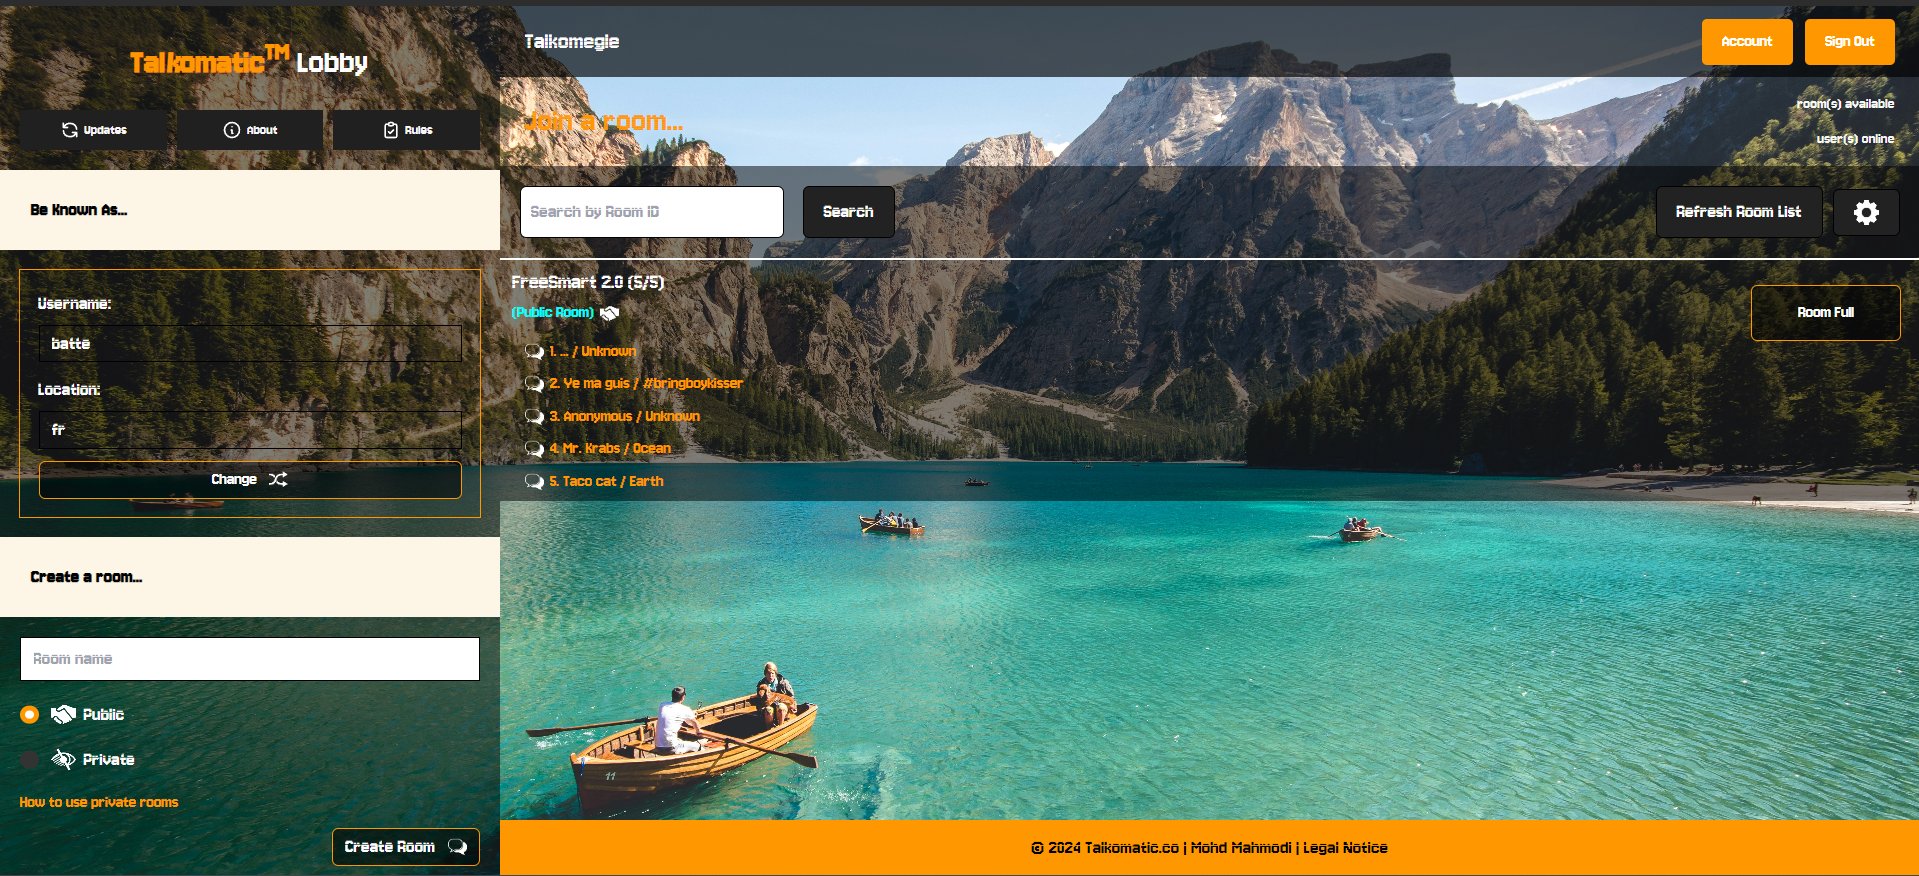
\includegraphics[width=1\linewidth]{6.png}
    \caption{Theme with transparent background colour}
    \label{fig:enter-label}
\end{figure}

\subsection{What are the numbers found in some variables?}

Not all variables are colours though. Some have a number (or multiple, or even multiple numbers with colours), and most of the time have a suffix like \texttt{px}, \texttt{s}, or even \texttt{rem}. This section will just explain what those measurements really mean.

The \texttt{px} suffix signifies a number of pixels. Some variables use a number of pixels to signify spacing of some text sizes and spacing for instance.

The \texttt{s} suffix means a number of seconds, a duration. The only case where this is really used is to control the speed at which transitions occur.

The \texttt{rem} suffix is the height of a "non-modified"\footnote{By "non-modified", I mean text not modified by CSS.} character. This means that you can position and size elements relative to the text size. This is mainly used to scale big text to be 1.8x times bigger than the normal text size.

\subsection{Custom fonts}

Ever got tired of the base font used in Talkomatic? Well, fear no more (if you were scared that is, for some reason), with the magic of typefaces/fonts, by modifying the 4th line of the file (\texttt{--font-family: 'Consolas', monospace;}). The value of the \texttt{font-family} variable is divided into two parts, your wanted font, and something called a web-safe font\footnote{The font used by browsers if your main font somehow does not load properly. Here's the list of them: \url{https://www.w3schools.com/cssref/css_websafe_fonts.php}}. If you for example, wanted to change your theme font to Comic Sans for some reason, here you go:
\begin{tcolorbox}[colback=green!5!white,colframe=green!75!black,title=Custom font example]
  \texttt{--font-family: "Comic Sans MS", sans-serif;}
\end{tcolorbox}
This line changes the default font to Comic Sans, and uses a sans-serif "backup" web-safe font. This Comic Sans font would usually load like that, since your operating system\footnote{If you don't know what that is, it's basically the program that gives your computer has an interface, files, apps, etc.} likely has it stored, and can use it on the go. However, for more \textit{unknown} fonts, this is not always the case. With the \texttt{@import} symbol\footnote{Do not forget to always put the import symbols at the top of your file, before the \texttt{:root} segment.} though, you can import any font easily (as long as it is available on the web). Here's an example of it (not a real link to a font):
\begin{tcolorbox}[colback=green!5!white,colframe=green!75!black,title=@import at-rule example]
  \texttt{@import url("https://example.com/some-font");}
\end{tcolorbox}

In my opinion, the best way to get those \texttt{@import} lines to paste so you can get new fonts, is \href{https://fonts.google.com}{Google Fonts}. (there can also be some other sources, and only from reputable sources. also, I'm not sponsored ;))
On Google Fonts, simply search up a font you like, and click on "Get Font" (see Figure 7).
\begin{figure}
    \centering
    
\includegraphics[width=1\linewidth]{7.png}
    \caption{Google Fonts example}
    \label{fig:enter-label}
\end{figure}
Afterwards, click on "Get Embed Code", choose "\texttt{@import}", and copy the middle line (that has \texttt{@import}). (example in Figure 8)
\begin{figure}
    \centering
    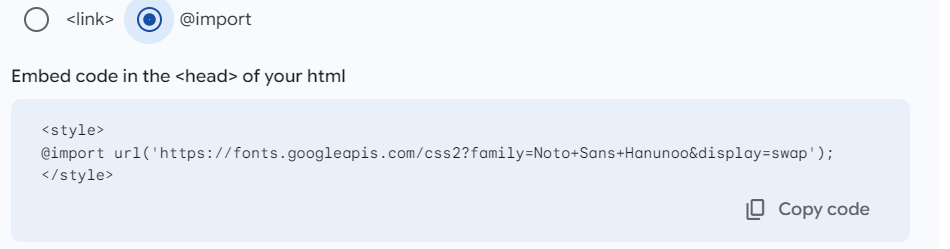
\includegraphics[width=1\linewidth]{8.png}
    \caption{Getting the embed code}
    \label{fig:enter-label}
\end{figure}
Now with my example, all that is left to do is this:
\begin{tcolorbox}[colback=green!5!white,colframe=green!75!black,title=Integrating the font]
  \texttt{--font-family: "Noto Sans Hanunoo", sans-serif;}
\end{tcolorbox}

\subsection{Using images}

Do you \textit{also} fear plain backgrounds? Well thankfully, this time Mohd Mahmodi\footnote{\url{talkomatic.co}'s owner} has a solution. In this \href{https://discord.com/channels/1252540401072607355/1277166363051556965}{discord forum thread}, there's already a background image template and tutorial, that even supports transparency!

\subsection{What are addons?}

An addon is another CSS file that you can upload with a main theme. Sounds confusing? Imagine a theme with a red background. Now, this theme has 2 addons\footnote{Think of addons like variants.}, one that changes the background to green, and the second changes the background to blue.

Let's try coding that up! \texttt{red-background.css} is our main theme file here. In the example below, only the third line that changes the background to red is shown. The rest of the file is exactly the same as the template's.

\begin{tcolorbox}[colback=green!5!white,colframe=green!75!black,title=red-background.css]
  \texttt{--body-bg: \#ff0000;}
\end{tcolorbox}

Now, let's see how the 2 other addons work:

\begin{tcolorbox}[colback=green!5!white,colframe=green!75!black,title=green-addon.css]
  \texttt{
  :root \{ --body-bg: \#00ff00; \}
  }
\end{tcolorbox}

\begin{tcolorbox}[colback=green!5!white,colframe=green!75!black,title=blue-addon.css]
  \texttt{
  :root \{ --body-bg: \#0000ff; \}
  }
\end{tcolorbox}

Addons are just normal theme files, except they keep all the unmodified features in the addon, and just overwrites new stuff over the normal theme.

Let's see what a combined theme would look like, and a normal theme:

\begin{tcolorbox}[colback=green!5!white,colframe=green!75!black,title=Uncombined theme]
  \texttt{:root \{ \newline
  /* General */ \newline
  --body-bg: \#ffffff; \newline
  --font-family: 'Consolas', monospace; \newline
  --font-size-base: 16px; \newline
  ... \newline \}}
\end{tcolorbox}

\begin{tcolorbox}[colback=green!5!white,colframe=green!75!black,title=Combined theme with green-addon.css]
  \texttt{:root \{ \newline
  /* General */ \newline
  \textcolor{green}{--body-bg: \#00ff00;} \newline
  --font-family: 'Consolas', monospace; \newline
  --font-size-base: 16px; \newline
  ... \newline \}}
\end{tcolorbox}

\begin{tcolorbox}[colback=green!5!white,colframe=green!75!black,title=Combined theme with blue-addon.css]
  \texttt{:root \{ \newline
  /* General */ \newline
  \textcolor{green}{--body-bg: \#0000ff;} \newline
  --font-family: 'Consolas', monospace; \newline
  --font-size-base: 16px; \newline
  ... \newline \}}
\end{tcolorbox}

Addons simply replace variables from the original, allowing for small tweaks or variants, and customization.


\section{Epilogue (now what?)}

Well, if you read all of this to end, congrats (you probably have a good patience and attention span). Now, as the section name suggests; what next? This guide is only to get you started in some theme customization, but CSS is more than that. You can modify the layout even more, and your own text effects, have a complete overhaul of how Talkomatic looks! There is only much that I can fit in a short little beginner-friendly guide. Most of even more advanced theme creation like text effects are beyond the scope of this, and require some knowledge in CSS. That being said, if you want to go \textit{above and beyond}, I recommend checking out the \href{https://www.w3schools.com/css/}{W3Schools CSS tutorial}, which is really beginner friendly, and will give you a more solid understanding of CSS. Complicated stuff aside, if you read this even a little bit, thank you so much, because it made a few hours that I wasted on this, a little bit less wasteful. Thank you for using \url{talkomatic.co}, for reading this guide, for being part of the community, and thanks \LaTeX\footnote{This guide is completely open-source (meaning the code for this is available for free) at \url{https://github.com/BatteRaquette581/The-Guide-To-Making-talkomatic.co-Themes}!} for powering this guide. ;-)


\end{document}
